\begin{chapter}{Physical Implementation}
\label{chap_04:physicalImplem}

\subsection{Mechanical structure}
Moving from the theoretical model and control design to the actual implementation. We designed the structure of the robot using the CAD Solidworks
and produced it using a 3D printer. 
The main structure of the robot is made of PETG material, while the wheels are made of TPU to ensure better grip on the ground.

\begin{figure}[h]
    \centering
    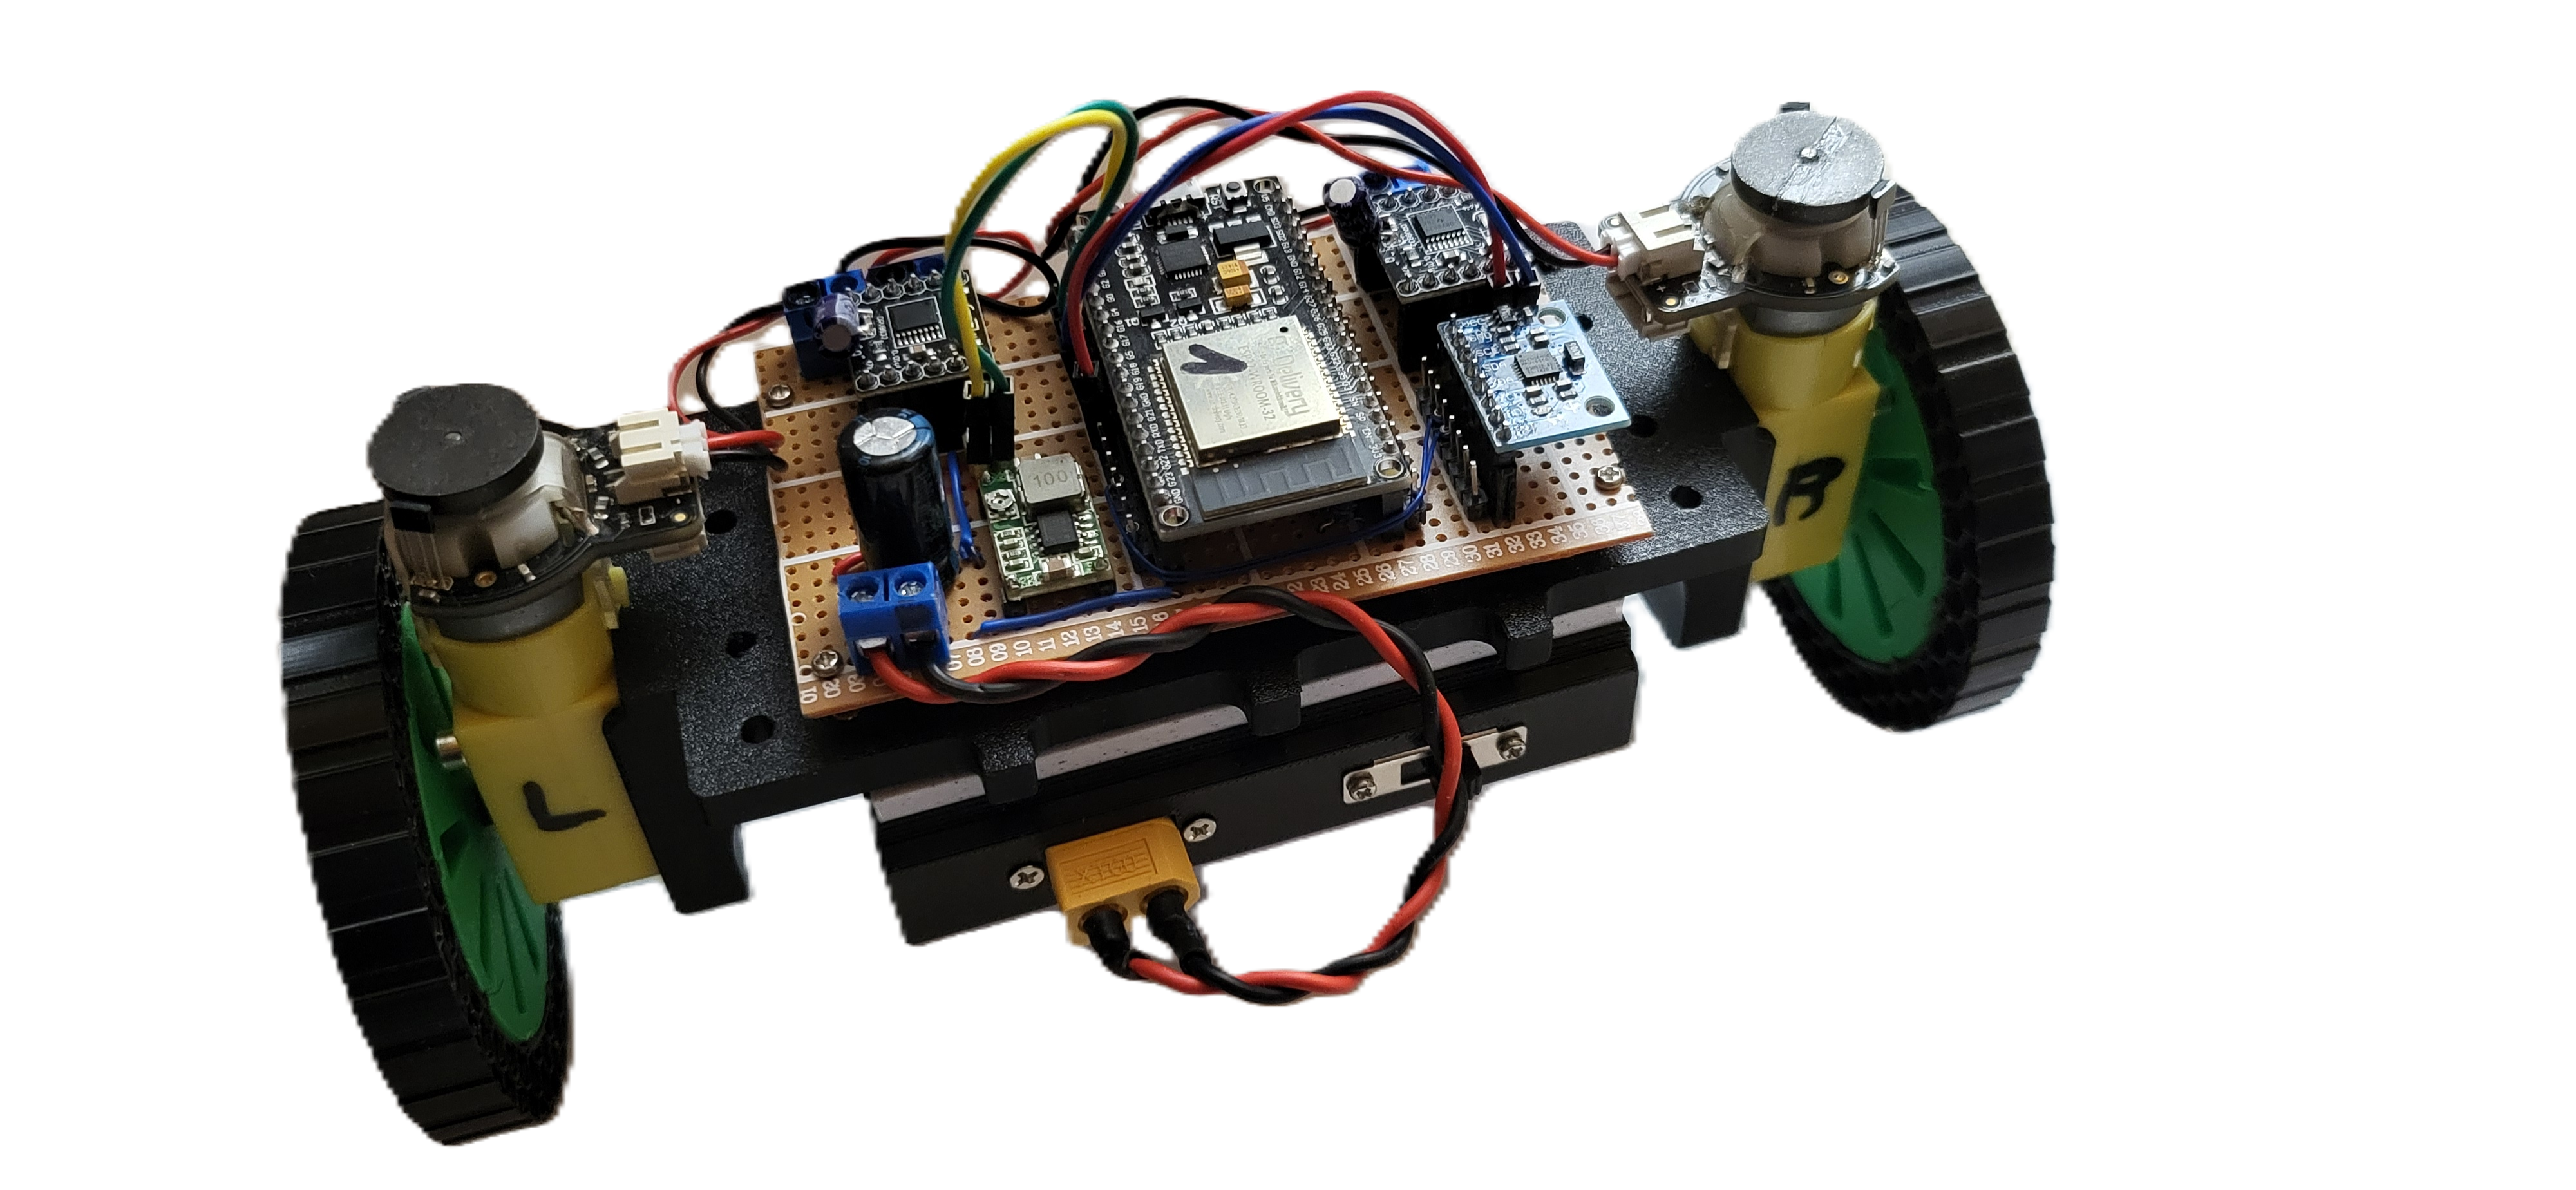
\includegraphics[width=0.7\linewidth]{figures/04_implementation/jamal_01.png}
    \caption{Robot}
\label{fig:04_robot_strucuture}
\end{figure}

The complete structure is shown in Figure \ref{fig:04_robot_strucuture}, while \ref{fig:04_tires} shows different tire designs.

\begin{figure}[h]
    \centering
    \includegraphics[width=0.7\linewidth]{figures/04_implementation/tires.jpg}
    \caption{Different tire geometries tried for the robot. Left to right for lower infill density and higher friction coefficient}
\label{fig:04_tires}
\end{figure}

During some initial tests it was found that the limited weight of the robot was not enough to ensure it stayed well connected to the ground. To reduce the loss of traction on smooth surfaces, we had to change the tire structure. Unfortunately, changing material is not really feasible, as not many flexible filaments options are available other than 95A TPU. Instead, we changed the tire density, lowering sparse infill to 15\% and eventually 8\%.
To further add flexibility, the shoulder of the tire had to be increased too, resulting in a larger diameter. Thanks to this simple solution, the tire deforms enough under torque to stay well connected to smooth tabletops.

\subsection{PID adjustments}

The PID controller parameters obtained in Chapter \ref{chap_02:modelling} are a good starting point for the real 
implementation, but due to the simplifications made in the model and the non-idealities of the real components,
it is necessary to adjust them experimentally.
After several tests, the final parameters used in the firmware are:
\begin{itemize}
    \item $K_P = 10$
    \item $K_I = 0.02$
    \item $K_D = 0.4$
\end{itemize}
These values ensure a good balancing performance, with a fast response to disturbances and minimal oscillations around the vertical position.

\subsection{Other adjustments}
Other parameters that needed to be adjust experimentally were for example the full-scale range of the accelerometer:
we experinced that setting it to $\pm 4g$ ensured a good compromise between sensitivity and range of measurement, while 
setting it to $\pm 2g$ resulted in a high noise measurement.

In order to use the robot without the need of a computer connected via USB, we inserted a simple buck converter to power the ESP32
from the batteries.
\end{chapter}